\documentclass[journal = jpccck, manuscript = article]{achemso}
\setkeys{acs}{usetitle = true}
\usepackage{achemso}
\usepackage{natbib}
\usepackage{multirow}
\usepackage{wrapfig}
\usepackage{fixltx2e}
%\mciteErrorOnUnknownfalse

\usepackage[version=3]{mhchem}  % this is a great package for formatting chemical reactions
\usepackage{url}


\title{Do the facets of ice $I_\mathrm{h}$ crystals have different
  friction coefficients?  Simulating shear in ice/water interfaces}

\author{P. B. Louden}
\author{J. Daniel Gezelter}
\email{gezelter@nd.edu}
\affiliation[University of Notre Dame]{251 Nieuwland Science Hall\\
  Department of Chemistry and Biochemistry\\ University of Notre
  Dame\\ Notre Dame, Indiana 46556}

\keywords{}

\begin{document}

\begin{abstract}
We have investigated the structural properties of the basal and
prismatic facets of an SPC/E model of the ice Ih / water interface
when the solid phase is being drawn through liquid water (i.e. sheared
relative to the fluid phase). To impose the shear, we utilized a
reverse non-equilibrium molecular dynamics (RNEMD) method that creates
non-equilibrium conditions using velocity shearing and scaling (VSS)
moves of the molecules in two physically separated slabs in the
simulation cell. This method can create simultaneous temperature and
velocity gradients and allow the measurement of friction transport
properties at interfaces. We present calculations of the interfacial
friction coefficients and the apparent independence of shear rate on
interfacial width and show that water moving over a flat ice/water
interface is close to the no-slip boundary condition.
\end{abstract}

\newpage

\section{Introduction}
%-----Outline of Intro---------------
% in general, ice/water interface is important b/c ....
% here are some people who have worked on ice/water, trying to understand the processes above ....
% with the recent development of VSS-RNEMD, we can now look at the shearing problem
% talk about what we will present in this paper
% -------End Intro------------------


%Gay02: cites many other ice/water papers, make sure to cite them.

Understanding the ice/water interface is essential for explaining complex processes such as nucleartion and crystal growth\cite{Han92,Granasy95,Vanfleet95}, crystal melting\cite{Weber83,Han92,Sakai96,Sakai96B}, and biological interfacial processes, such as the antifreeze protein found in winter flounder\cite{Wierzbicki07, Chapsky97}. 

Haymet \emph{et al.} have done extensive work on ice Ih, including characterizing and determining the width of the ice/water interface for the SPC, SPC/E, CF1, and TIP4P models for water. \cite{Karim87,Karim88,Karim90,Hayward01,Bryk02,Hayward02,Gay02} More recently, Haymet \emph{et al.} have been investigating the effects cations and anions have on crystal nucleation\cite{Bryk04,Smith05,Wilson08,Wilson10}. Nada \emph{et al.} have also studied the ice/water interface\cite{Nada95,Nada00,Nada03,Nada12}. They have found that the different facets of ice Ih have different growth rates, primarily, that the prismatic facet grows faster than the basal facet due to the mechanism of the crystal growth being the reordering of the hydrogen bonding network\cite{Nada05}. Other groups \cite{Baez95,Arbuckle02,}.



%Other people looking at the ice/water interface, bio, crystal nucleation, kinetics, etc. 
%Geologists are concerned with the flow of water over ice
%Antifreeze protein in fish--Haymet's group has cited this before

%Paragraph explaining why the ice/water interface is important
%Paragraph on what other people have done / lead into what hasn't been done
%Paragraph on what I'm going to do 




With the recent development of velocity shearing and scaling reverse non-equilibrium molecular dynamics (VSS-RNEMD), it is now possible to calculate transport properties from heterogeneous systems.\cite{Kuang12} This method can create simultaneous temperature and velocity gradients and allow the measurement of friction and thermal transport properties at interfaces. This allows for the study of the width of the ice/water interface as the ice is sheared through the liquid, while imposing a thermal gradient to prevent frictional heating of the interface. 

In this paper, we investigate the width and the friction coefficient of the ice/water interface as the ice is sheared through the liquid. 

\section{Methodology}

\subsection{Stable ice I$_\mathrm{h}$ / water interfaces}

The structure of ice I$_\mathrm{h}$ is well understood; it
crystallizes in a hexagonal space group P$6_3/mmc$, and the hexagonal
crystals of ice have two faces that are commonly exposed, the basal
face $\{0~0~0~1\}$, which forms the top and bottom of each hexagonal
plate, and the prismatic $\{1~0~\bar{1}~0\}$ face which forms the
sides of the plate. Other less-common, but still important, faces of
ice I$_\mathrm{h}$ are the secondary prism face, $\{1~1~\bar{2}~0\}$,
and the prismatic face, $\{2~0~\bar{2}~1\}$.

Ice I$_\mathrm{h}$ is normally proton disordered in bulk crystals,
although the surfaces probably have a preference for proton ordering
along strips of dangling H-atoms and Oxygen lone
pairs.\cite{Buch:2008fk}

For small simulated ice interfaces, it is useful to have a
proton-ordered, but zero-dipole crystal that exposes these strips of
dangling H-atoms and lone pairs.  Also, if we're going to place
another material in contact with one of the ice crystalline planes, it
is useful to have an orthorhombic (rectangular) box to work with.  A
recent paper by Hirsch and Ojam\"{a}e describes how to create
proton-ordered bulk ice I$_\mathrm{h}$ in alternative orthorhombic
cells.\cite{Hirsch04}

We have using Hirsch and Ojam\"{a}e's structure 6 which is an
orthorhombic cell ($P2_12_12_1$) that produces a proton-ordered
version of ice Ih.  Table \ref{tab:equiv} contains a mapping between
the Miller indices in the P$6_3/mmc$ crystal system and those in the
Hirsch and Ojam\"{a}e $P2_12_12_1$ system.

\begin{wraptable}{r}{3.5in}
\begin{tabular}{|ccc|} \hline
 & hexagonal & orthorhombic \\
 & ($P6_3/mmc$) & ($P2_12_12_1$) \\
 crystal face  & Miller indices & equivalent \\ \hline
basal & $\{0~0~0~1\}$ & $\{0~0~1\}$ \\
prism & $\{1~0~\bar{1}~0\}$ & $\{1~0~0\}$ \\
secondary prism & $\{1~1~\bar{2}~0\}$ & $\{1~3~0\}$ \\
pryamidal & $\{2~0~\bar{2}~1\}$ & $\{2~0~1\}$ \\ \hline
\end{tabular}
\end{wraptable}

Structure 6 from the Hirsch and Ojam\"{a}e paper has lattice
parameters $a = 4.49225$, $b = 7.78080$, $c = 7.33581$ and two water
molecules whose atoms reside at the following fractional coordinates:

\begin{wraptable}{r}{3.25in}
\begin{tabular}{|ccccc|}  \hline
atom label & type & x & y & z \\ \hline
O$_{a}$    & O & 0.75 & 0.1667 & 0.4375 \\
H$_{1a}$ & H & 0.5735 & 0.2202 & 0.4836 \\
H$_{2a}$ & H & 0.7420 & 0.0517 & 0.4836 \\
O$_{b}$    & O & 0.25 & 0.6667 & 0.4375 \\
H$_{1b}$ & H & 0.2580 & 0.6693 & 0.3071 \\
H$_{2b}$ & H & 0.4265 & 0.7255 & 0.4756 \\ \hline
\end{tabular}
\end{wraptable}

To construct the basal and prismatic interfaces, the crystallographic
coordinates above were used to construct an orthorhombic unit cell
which was then replicated in all three dimensions yielding a
proton-ordered block of ice I$_{h}$. To expose the desired face, the
orthorhombic representation was then cut along the ($001$) or ($100$)
planes for the basal and prismatic faces respectively.  The resulting
block was rotated so that the exposed faces were aligned with the $z$
axis normal to the exposed face.  The block was then cut along two
perpendicular directions in a way that allowed for perfect periodic
replication in the $x$ and $y$ axes, creating a slab with either the
basal or prismatic faces exposed along the $z$ axis.  The slab was
then replicated in the $x$ and $y$ dimensions until a desired sample
size was obtained.  

Although experimental solid/liquid coexistant temperature under normal
pressure are close to 273K, Haymet \emph{et al.} have done extensive
work on characterizing the ice/water
interface.\cite{Karim88,Karim90,Hayward01,Bryk02,Hayward02} They have
found for the SPC/E water model,\cite{Berendsen87} which is also used
in this study, the ice/water interface is most stable at
225$\pm$5K.\cite{Bryk02} To create a ice / water interface, a box of
liquid water that had the same dimensions in $x$ and $y$ was
equilibrated at 225 K and 1 atm of pressure in the NPAT ensemble (with
the $z$ axis allowed to fluctuate to equilibrate to the correct
pressure).  The liquid and solid systems were combined by carving out
any water molecule from the liquid simulation cell that was within 3
\AA\ of any atom in the ice slab.

Molecular translation and orientational restraints were applied in the
early stages of equilibration to prevent melting of the ice slab.
These restraints were removed during NVT equilibration, well before
data collection was carried out.

\subsection{Shearing ice / water interfaces without bulk melting}

As one drags a solid through a liquid, there will be frictional
heating that will act to melt the interface.  To study the frictional
behavior of the interface without causing the interface to melt, it is
necessary to apply a weak thermal gradient along with the momentum
gradient.  This can be accomplished with of the newly-developed
approaches to reverse non-equilibrium molecular dynamics (RNEMD).  The
velocity shearing and scaling (VSS) variant of RNEMD utilizes a series
of simultaneous velocity exchanges between two regions within the
simulation cell.\cite{Kuang12} One of these regions is centered within
the ice slab, while the other is centrally located in the liquid phase
region. VSS-RNEMD provides a set of conservation constraints for
simultaneously creating either a momentum flux or a thermal flux (or
both) between the two slabs.  Satisfying the constraint equations
ensures that the new configurations are sampled from the same NVE
ensemble as previously.

The VSS moves are applied periodically to scale and shift the particle
velocities ($\mathbf{v}_i$ and $\mathbf{v}_j$) in two slabs ($H$ and
$C$) which are separated by half of the simulation box,
\begin{displaymath}
\begin{array}{rclcl}

 & \underline{\mathrm{shearing}} & &
 \underline{~~~~~~~~~~~~\mathrm{scaling}~~~~~~~~~~~~} \\
\mathbf{v}_i \leftarrow & 
  \mathbf{a}_c\ & + & c\cdot\left(\mathbf{v}_i - \langle\mathbf{v}_c
  \rangle\right)  +  \langle\mathbf{v}_c\rangle \\
\mathbf{v}_j \leftarrow & 
  \mathbf{a}_h & + & h\cdot\left(\mathbf{v}_j - \langle\mathbf{v}_h
    \rangle\right) + \langle\mathbf{v}_h\rangle .

\end{array}
\end{displaymath}
Here $\langle\mathbf{v}_c\rangle$ and $\langle\mathbf{v}_h\rangle$ are
the center of mass velocities in the $C$ and $H$ slabs, respectively.
Within the two slabs, particles receive incremental changes or a
``shear'' to their velocities.  The amount of shear is governed by the
imposed momentum flux, $\mathbf{j}_z(\mathbf{p})$
\begin{eqnarray}
\mathbf{a}_c & = & - \mathbf{j}_z(\mathbf{p}) \Delta t / M_c \label{vss1}\\
\mathbf{a}_h & = & + \mathbf{j}_z(\mathbf{p}) \Delta t / M_h \label{vss2}
\end{eqnarray}
where $M_{\{c,h\}}$ is the total mass of particles within each of the
slabs and $\Delta t$ is the interval between two separate operations.

To simultaneously impose a thermal flux ($J_z$) between the slabs we
use energy conservation constraints,
\begin{eqnarray}
K_c - J_z\Delta t & = & c^2 (K_c - \frac{1}{2}M_c \langle\mathbf{v}_c
\rangle^2) + \frac{1}{2}M_c (\langle \mathbf{v}_c \rangle + \mathbf{a}_c)^2 \label{vss3}\\
K_h + J_z\Delta t & = & h^2 (K_h - \frac{1}{2}M_h \langle\mathbf{v}_h
\rangle^2) + \frac{1}{2}M_h (\langle \mathbf{v}_h \rangle +
\mathbf{a}_h)^2 \label{vss4}.
\label{constraint}
\end{eqnarray}
Simultaneous solution of these quadratic formulae for the scaling
coefficients, $c$ and $h$, will ensure that the simulation samples from
the original microcanonical (NVE) ensemble.  Here $K_{\{c,h\}}$ is the
instantaneous translational kinetic energy of each slab.  At each time
interval, it is a simple matter to solve for $c$, $h$, $\mathbf{a}_c$,
and $\mathbf{a}_h$, subject to the imposed momentum flux,
$j_z(\mathbf{p})$, and thermal flux, $J_z$, values.  Since the VSS
operations do not change the kinetic energy due to orientational
degrees of freedom or the potential energy of a system, configurations
after the VSS move have exactly the same energy (and linear
momentum) as before the move.

As the simulation progresses, the VSS moves are performed on a regular
basis, and the system develops a thermal and/or velocity gradient in
response to the applied flux.  In a bulk material it is quite simple
to use the slope of the temperature or velocity gradients to obtain
the thermal conductivity or shear viscosity.

The VSS-RNEMD approach is versatile in that it may be used to
implement thermal and shear transport simultaneously.  Perturbations
of velocities away from the ideal Maxwell-Boltzmann distributions are
minimal, as is thermal anisotropy.  This ability to generate
simultaneous thermal and shear fluxes has been previously utilized to
map out the shear viscosity of SPC/E water over a wide range of
temperatures (90~K) with a single 1 ns simulation.\cite{Kuang12}

Here we are using this method primarily to generate a shear between
the ice slab and the liquid phase, while using a weak thermal gradient
to maintaining the interface at the 225K target value.  This will
insure minimal melting of the bulk ice phase and allows us to control
the exact temperature of the interface.

\subsection{Computational Details}
All simulations were performed using OpenMD with a time step of 2 fs,
and periodic boundary conditions in all three dimensions. The systems
were divided into 100 artificial bins along the $z$-axis for the
VSS-RNEMD moves, which were attempted every 50 fs. The gradients were
allowed to develop for 1 ns before data collection was began. Once
established, snapshots of the system were taken every 1 ps, and the
average velocities and densities of each bin were accumulated every
attempted VSS-RNEMD move.

%A paragraph on the equilibration procedure of the system? Shenyu did some amount of equilibration to the files and then I was handed them. I performed 5 ns of NVT at 225K for both systems, then 5 ns of NVE at 225K for both systems, with no gradients imposed. 
%For the basal, once the thermal gradient was found which gave me the interfacial temperature I wanted (-2.0E-6 kcal/mol/A^2/fs), I equilibrated the file for 5 ns letting this gradient stabilize. Then I continued to use this thermal gradient as I imposed momentum gradients and watched the response of the interface.
%For the prismatic, a gradient was not found that would give me the interfacial temperature I desired, so while imposing a thermal gradient that had the interface at 220K, I raised the temperature of the system to 230K. This resulted in a thermal gradient which gave my interface at 225K, equilibrated for ins NVT, then ins NVE while this gradient was still imposed, then I began dragging.
%I have run each system for 1 ns under PTgrads to allow them to develop, then ran each system for an additional 2 ns in segments of 0.5 ns in order to calculate statistics of the calculated values.

\subsection{Measuring the Width of the Interface}
In order to characterize the ice/water interface, the local
tetrahedral order parameter as described by Kumar\cite{Kumar09} and
Errington\cite{Errington01} was used. The local tetrahedral order
parameter, $q$, is given by
\begin{equation}
q_{k} \equiv 1 -\frac{3}{8}\sum_{i=1}^{3} \sum_{j=i+1}^{4} \Bigg[\cos\psi_{ikj}+\frac{1}{3}\Bigg]^2
\end{equation}
where $\psi_{ikj}$ is the angle formed by the oxygen sites on molecule $k$, and the oxygen site on its two closest neighbors, molecules $i$ and $j$. The local tetrahedral order parameter function has a range of (0,1), where the larger the value $q$ has the more tetrahedral the ordering of the local environment is. A $q$ value of one describes a perfectly tetrahedral environment relative to it and its four nearest neighbors, and the parameter's value decreases as the local ordering becomes less tetrahedral.

%If the central water molecule has a perfect tetrahedral geometry with its four nearest neighbors, the parameter goes to one, and decreases to zero as the geometry deviates from the ideal configuration.

The system was divided into 100 bins along the $z$-axis, and a $q$ value was determined for each snapshot of the system for each bin. The $q$ values for each bin were then averaged to give an average tetrahedrally profile of the system about the $z$- axis. The profile was then fit with a hyperbolic tangent function given by 
\begin{equation}
q_{z}=q_{liq}+\frac{q_{ice}-q_{liq}}{2}(\tanh(\alpha(z-I_{L,m}))-\tanh(\alpha(z-I_{R,m})))
\end{equation}
where $q_{liq}$ and $q_{ice}$ are fitting parameters for the local tetrahedral order parameter for the liquid and ice, $\alpha$ is proportional to the inverse of the width of the interface, and $I_{L,m}$ and $I_{R,m}$ are the midpoints of the left and right interface. During the simulations where a kinetic energy flux was imposed, there was found to be a thermal influence in the liquid phase region of the tetrahedrally profile due to the thermal gradient developed in the system. To maximize the fit of the interface, another term was added to the hyperbolic tangent fitting function,
\begin{equation}
q_{z}=q_{liq}+\frac{q_{ice}-q_{liq}}{2}(\tanh(\alpha(z-I_{L,m}))-\tanh(\alpha(z-I_{R,m})))+\beta|(z-z_{mid})|
\end{equation}
where $\beta$ is a fitting parameter and $z_{mid}$ is the midpoint of the z dimension of the simulation box. 


\section{Results and discussion}

%Images to include: 3-long comic strip style of <Vx>, T, q_z as a function of z for the basal and prismatic faces. q_z by z with fit for basal and prismatic. interface width as a function of deltaVx (shear rate) with basal and prismatic on the same plot, error bars in the x and y. <Vx> by flux with basal and prismatic on same graph, back out slope from xmgr and error in slope to get lambda, friction coefficient of interface.

In Figures \ref{fig:bComic} and \ref{fig:pComic} we see the $z$-dimensional profiles for several parameters for the basal and prismatic systems respectively. In panel (a) of the figures we see the tetrahedrality profile of the systems (black circles). In the liquid region of the system, the local tetrahedral order parameter is approximately 0.75. In the solid region, the parameter is approximately 0.94, indicating a more tetrahedral structure of the water molecules. The hyperbolic tangent function used to fit the tetrahedrality profiles can be found in red and the verticle dotted lines denote the midpoint of the interfaces. The weak thermal gradient applied to the systems in order to keep the interface at a stable temperature, 225$\pm$5K, can be seen in panel (b).  Lastly, the velocity gradient across the systems can be seen in panel (c). From panel (c), we can see liquid phase water molecules 5 to 12 \AA\ from the midpoint of the basal and prismatic interfaces are being dragged along with the ice block. This indicates that the shearing of ice water is in the stick boundary condition.   

\begin{figure}
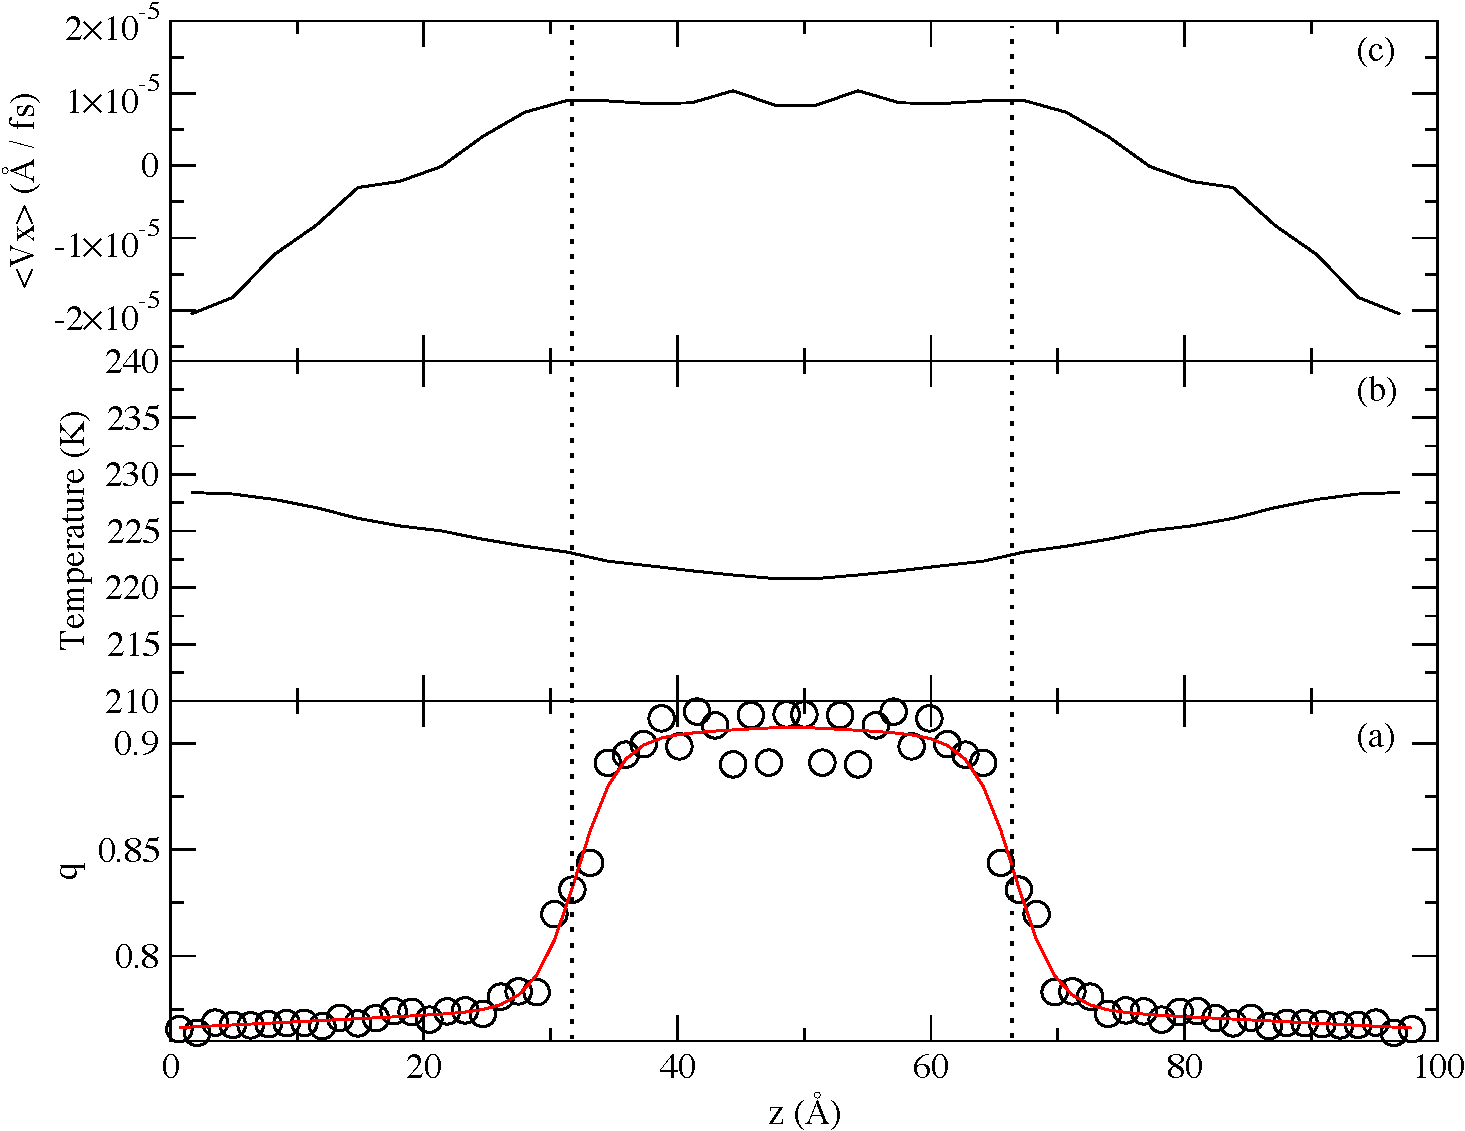
\includegraphics[width=\linewidth]{bComicStrip}
\caption{\label{fig:bComic} The basal system: (a) The local tetrahedral order parameter,$q$, (black circles) fit by a hyperbolic tangent (red line), (b) the thermal gradient imposed on the system to maintain a stable interfacial temperature, and (c) the velocity gradient imposed on the system. The verticle dotted lines indicate the midpoint of the interfaces.}
\end{figure}

%(a) The local tetrahedral order parameter across the z-dimension of the system (black circles) fit by a hyperbolic tangent (red line). (b) The thermal gradient imposed on the system to maintain a stable interfacial temperature. (c) The velocity gradient imposed on the system. The verticle dotted lines indicate the midpoint of the interfaces.

\begin{figure}
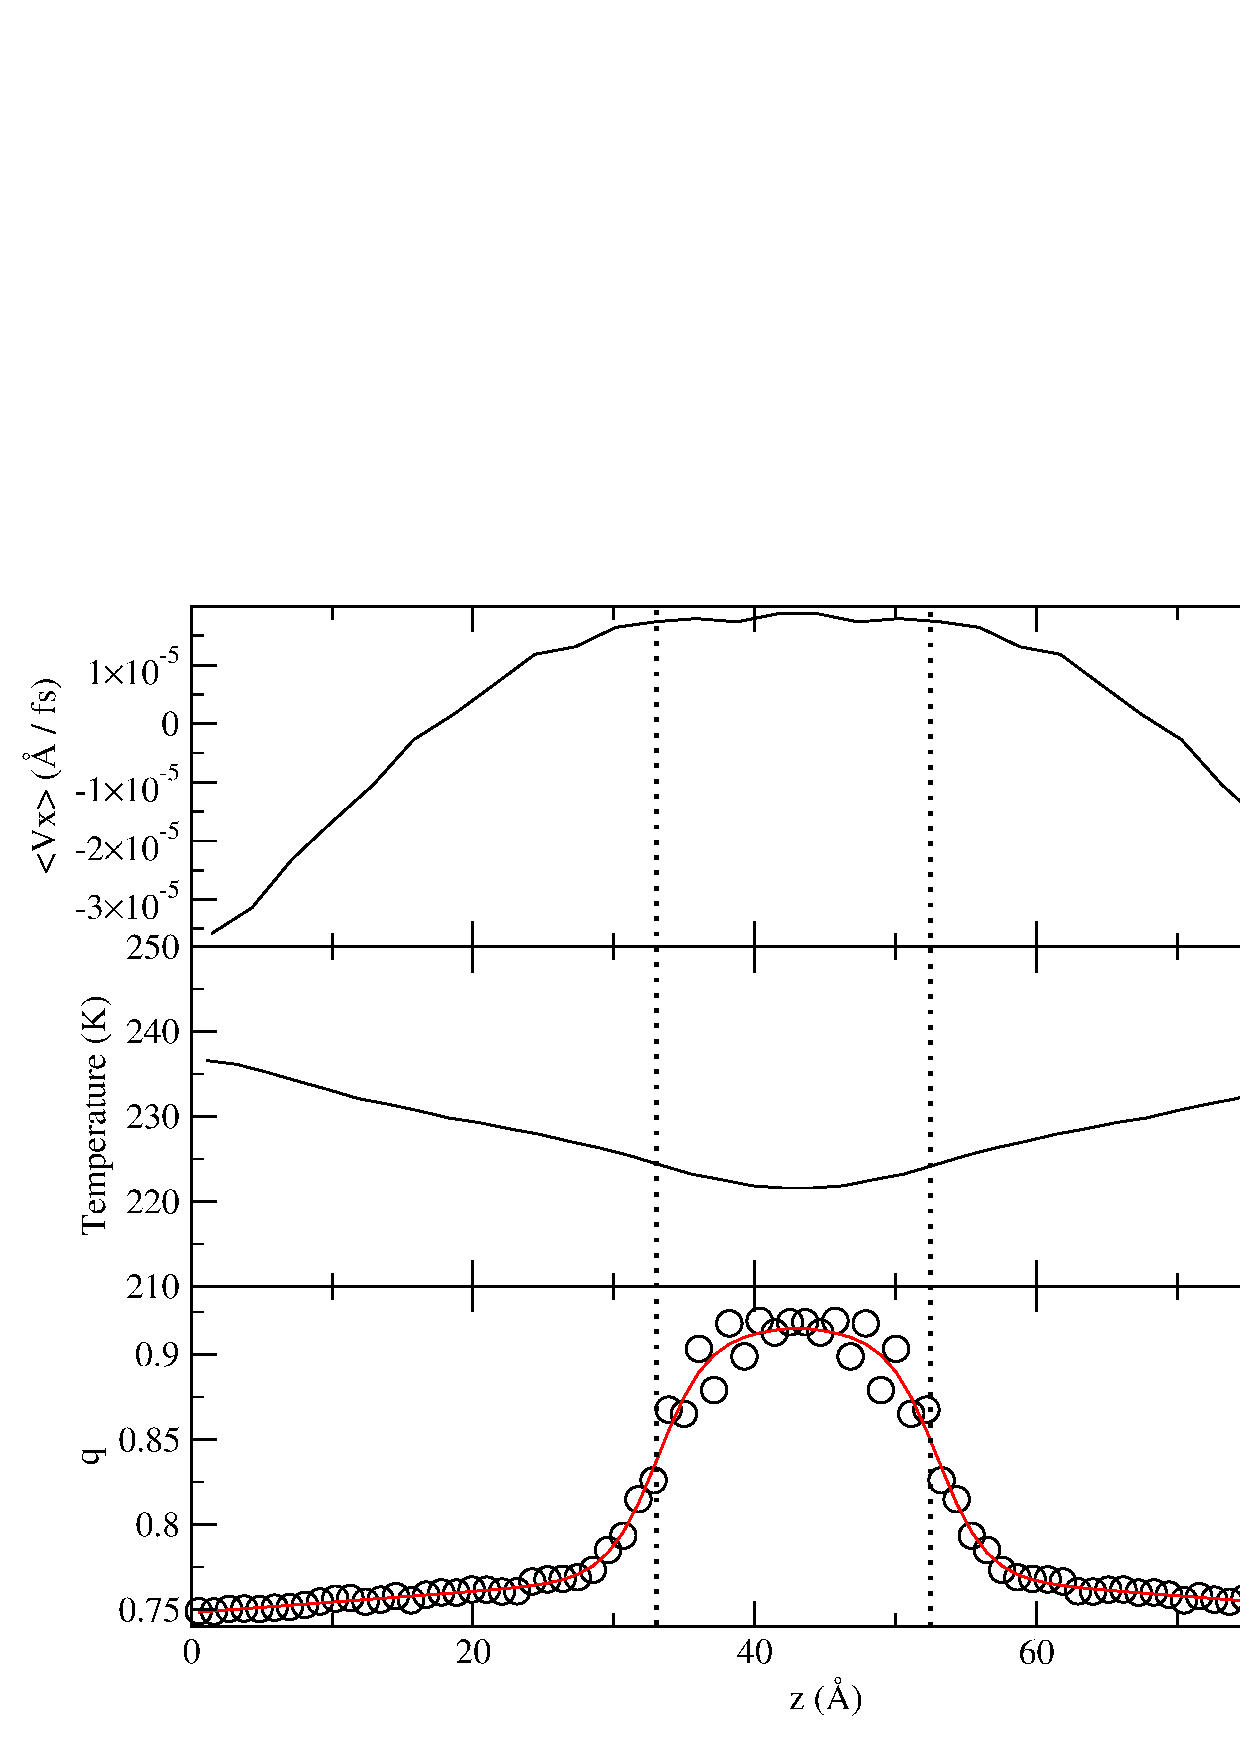
\includegraphics[width=\linewidth]{pComicStrip}
\caption{\label{fig:pComic} The prismatic system: (a) The local tetrahedral order parameter,$q$, (black circles) fit by a hyperbolic tangent (red line), (b) the thermal gradient imposed on the system to maintain a stable interfacial temperature, and (c) the velocity gradient imposed on the system.The verticle dotted lines indicate the midpoint of the interfaces.}
\end{figure}


\subsection{Interfacial Width}
%For the basal and prismatic systems, the ice blocks were sheared through the water at varying rates while an imposed thermal gradient kept the interface at the stable temperature range as described by Byrk and Haymet. 
We found the interfacial width for the basal and prismatic systems to be 3.2$\pm$0.4 \AA\ and 3.6$\pm$0.2 \AA\ with no applied momentum flux. Over the range of shear rates investigated, 0.6$\pm$0.3 ms\textsuperscript{-1} to 5.3$\pm$0.5 ms\textsuperscript{-1} for the basal system and 0.9$\pm$0.2 ms\textsuperscript{-1} to 4.5$\pm$0.1 ms\textsuperscript{-1}, there was no appreciable change in the interface width found. The calculated values for the interfacial width over all shear rates investigated contained the control values within their error bars.

%Need to reword the following paragraph
Beaglehole and Wilson have measured the ice/water interface to have a thickness approximately 10-20 \AA\ for both the basal and prismatic face of ice by ellipticity measurements \cite{Beaglehole93}. Haymet \emph{et al.} agrees with these measurements, our results do not. We are using a  parameter from the hyperbolic tangent fit of the local tetrahedrality order parameter to determine the interfacial width, whereas Haymet and co-workers use the 10-90 widths of the translational, average density, diffusion, and orientational decay times \cite{Hayward01}.

\subsection{Coefficient of Friction of the Interface}
As the ice is sheared through the liquid, there will be a friction between the ice and the interface. Balasubramanian has shown how to calculate the coefficient of friction for a solid-liquid interface. \cite{Balasubramanian99}
\begin{equation}
%<F_{x}^{w}>_{NE}(t)=-S\lambda_{wall}v_{x}(y_{wall})
\langle F_{x}^{w}\rangle(t)=-S\lambda_{wall}v_{x}(y_{wall})
\end{equation}
In this equation, $F_{x}^{w}$ is the total force of all the atoms acting on the fluid, $S$ is the surface area the force is being applied upon, and $\lambda_{wall}$ is the coefficient of friction of the interface. Since the imposed momentum flux, $J_{z}(p_{x})$, is known in the VSS-RNEMD simulations, and the $wall$ is the ice block in our simulations, the above equation can be rewritten as 
\begin{equation}
J_{z}(p_{x})=-\lambda_{ice}v_{x}(y_{ice}).
\end{equation}

In Figure \ref{fig:CoeffFric}, the average velocity of the ice is plotted against the imposed momentum flux for the basal (black circles) and prismatic (red circles) systems. From the equation above, the slope of the linear fit of the data is $\lambda_{wall}$. The coefficient of friction of the interface for the basal face was calculated to be 11.0 $\pm$ 0.4 \AA\textsuperscript{-2}fs\textsuperscript{-1}, and the $\lambda_{wall}$ for the prismatic face was determined to be 19.9, $\pm$ 0.5 \AA\textsuperscript{-2}fs\textsuperscript{-1}.  

%Ask dan about truncating versus rounding the values for lambda.
%The coefficient of friction of the interface for the basal face was calculated to be 11.02808 $\pm$  0.4489844 \AA^{-2}fs^{-1}, and the $\lambda_{wall}$ for the prismatic face was determined to be 19.95948, $\pm$ 0.5370894 \AA^{-2}fs^{-1}. 
\begin{figure}
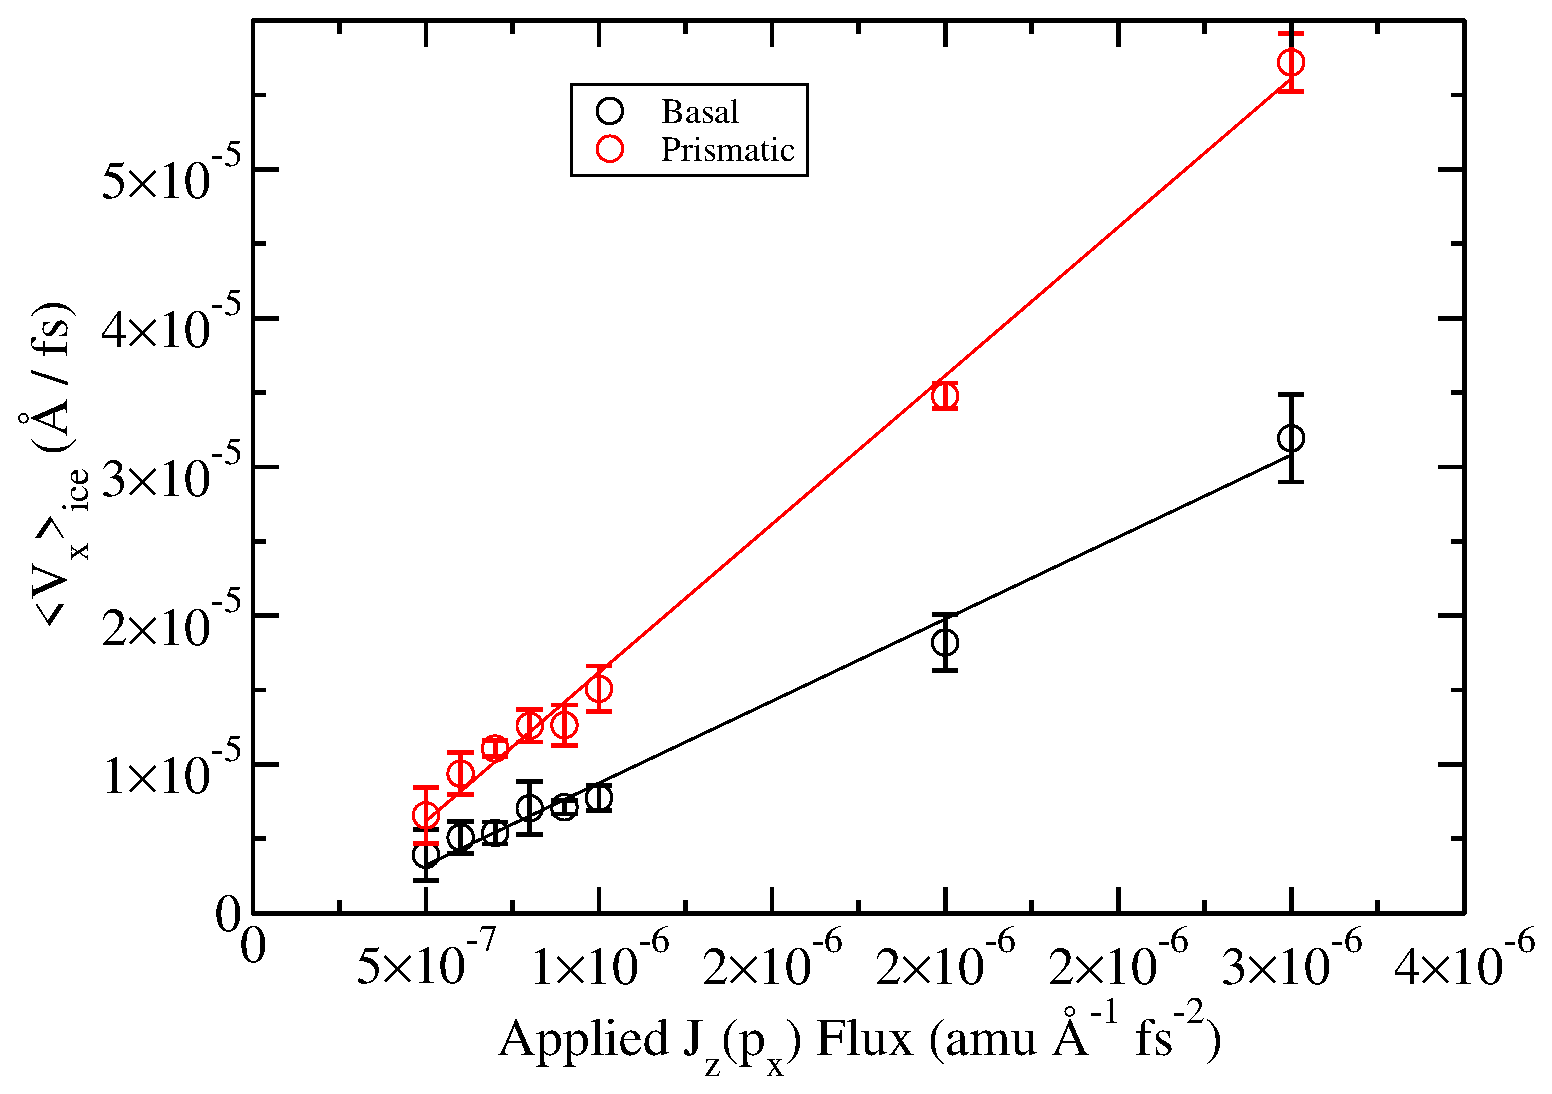
\includegraphics[width=\linewidth]{CoeffFric}
\caption{\label{fig:CoeffFric} The average velocity of the ice for the basal (black circles) and prismatic (red circles) systems as a function off applied momentum flux. The slope of the fit line   }
\end{figure}

\section{Conclusion}
Here we have simulated the basal and prismatic facets of an SPC/E model of the ice Ih / water interface. Using VSS-RNEMD, the ice was sheared relative to the liquid while imposed thermal gradients kept the interface at a stable temperature. Caculation of the local tetrahedrality order parameter has shown an appearant independence of the shear rate on the interfacial width. The coefficient of friction of the interface was also calculated for each of the facets. The $\lambda_{wall}$ for the basal face was calculated to be 11.0 $\pm$ 0.4 \AA\textsuperscript{-2}fs\textsuperscript{-1}, and 19.9, $\pm$ 0.5 \AA\textsuperscript{-2}fs\textsuperscript{-1} for the prismatic facet. For both facets, the shearing ice water was found to be in the no-slip boundary condition.  


\begin{acknowledgement}
  Support for this project was provided by the National Science
  Foundation under grant CHE-0848243. Computational time was provided
  by the Center for Research Computing (CRC) at the University of
  Notre Dame.
\end{acknowledgement}

\newpage
\bibstyle{achemso}
\bibliography{iceWater}

\begin{tocentry}
\begin{wrapfigure}{l}{0.5\textwidth}
\begin{center}
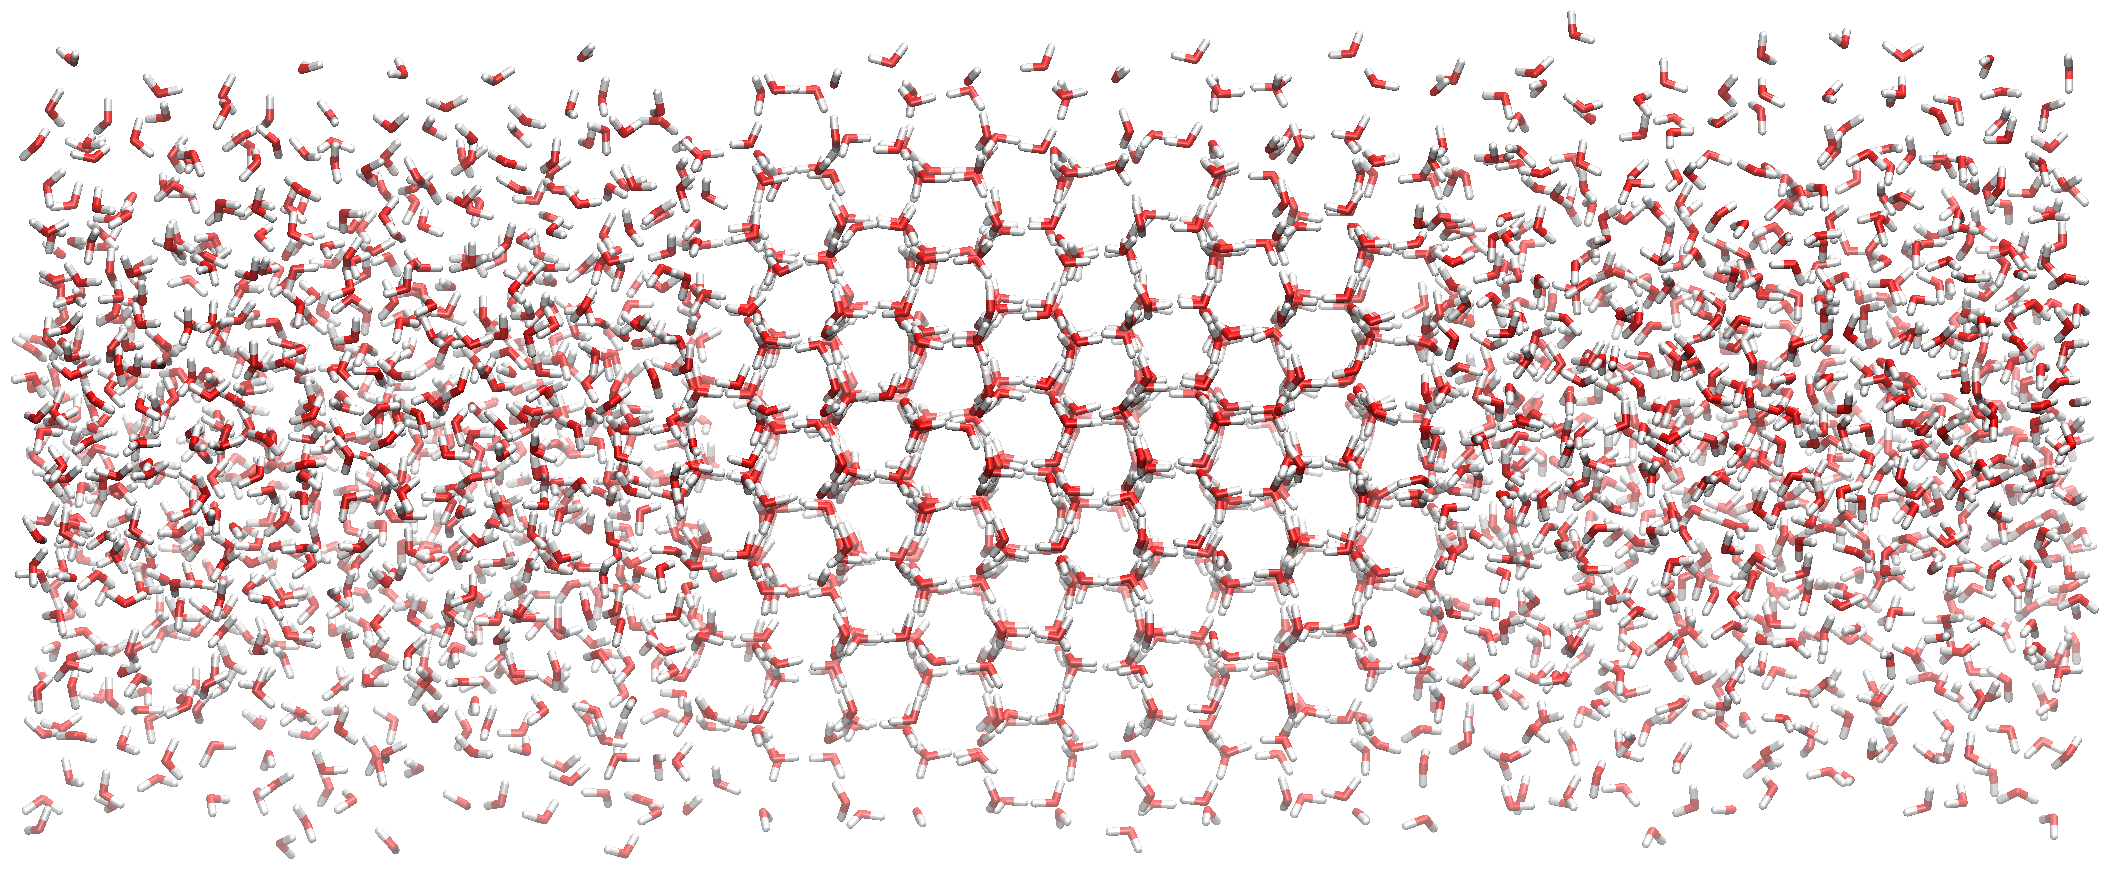
\includegraphics[width=\linewidth]{SystemImage.png}
\end{center}
\end{wrapfigure}
An image of our system.
\end{tocentry}

\end{document}

% basal: slope=11.02808, error in slope = 0.4489844
%prismatic: slope = 19.95948, error in slope  = 0.5370894
